\chapter{I-Mode Pedestal Stability Modeling}\label{ch:ImodeModeling}

Large, uncontrolled Edge-Localized Modes (ELMs -- see \cref{sec:hcr_elmy}) in ITER-scale operation are expected to drive unacceptable levels of pulsed heat loading and erosion damage to plasma-facing materials \cite{Loarte2003,Federici2003}.  As such, avoiding or mitigating large ELMs is a major focus of research in high-performance regimes, including active ELM control (\cref{subsec:hcr_elmy_control}) and inherently ELM-suppressed regimes (\cref{sec:hcr_elmsuppressed}).  To these we add the I-mode (\cref{sec:hcr_imode}), which appears to be naturally stable against large, deleterious ELMs in addition to its other beneficial properties (see \cref{ch:ImodePedestal}).

Confidence in plans for high-performance operation on ITER- and reactor-scale devices requires a predictive model for the pedestal structure and stability, to optimize fusion performance and ELM control or avoidance.  Recent cooperative efforts among theory, modeling, and experiment \cite{Groebner2013} have resulted in such a model for ELMy H-modes, termed EPED \cite{Snyder2009,Snyder2011}, detailed in \cref{sec:mod_eped}.  The EPED model combines constraints from peeling-ballooning MHD stability (\cref{sec:mod_pb}) \cite{Wilson2002,Snyder2004,Wilson2006}\gnote{cites?} and kinetic-ballooning turbulence (\cref{sec:mod_turbulence}) \cite{Snyder1999,Candy2005,Snyder2001}.  The EPED model has been successfully implemented in ELMy H-mode on a number of machines, including DIII-D \cite{Snyder2009,Snyder2011}, JT-60U \cite{Snyder2009}, C-Mod \cite{Walk2012}, and KSTAR \cite{Han2013}, as well as in QH-mode \cite{Snyder2012}; small/no-ELM regimes (EDA H-mode, type-II and type-III ELMy H-modes) have been shown to be stable against the drive identified in the EPED model \cite{Snyder2009}.

In this chapter, we apply the EPED approach to I-mode, examining the stability of the I-mode pedestal against peeling-ballooning MHD and kinetic-ballooning turbulence.

\section{MHD Stability -- ELITE}\label{sec:imode_elite}

\begin{figure}[p]
 \pushtooutside
 \ffigbox[\FBwidth]{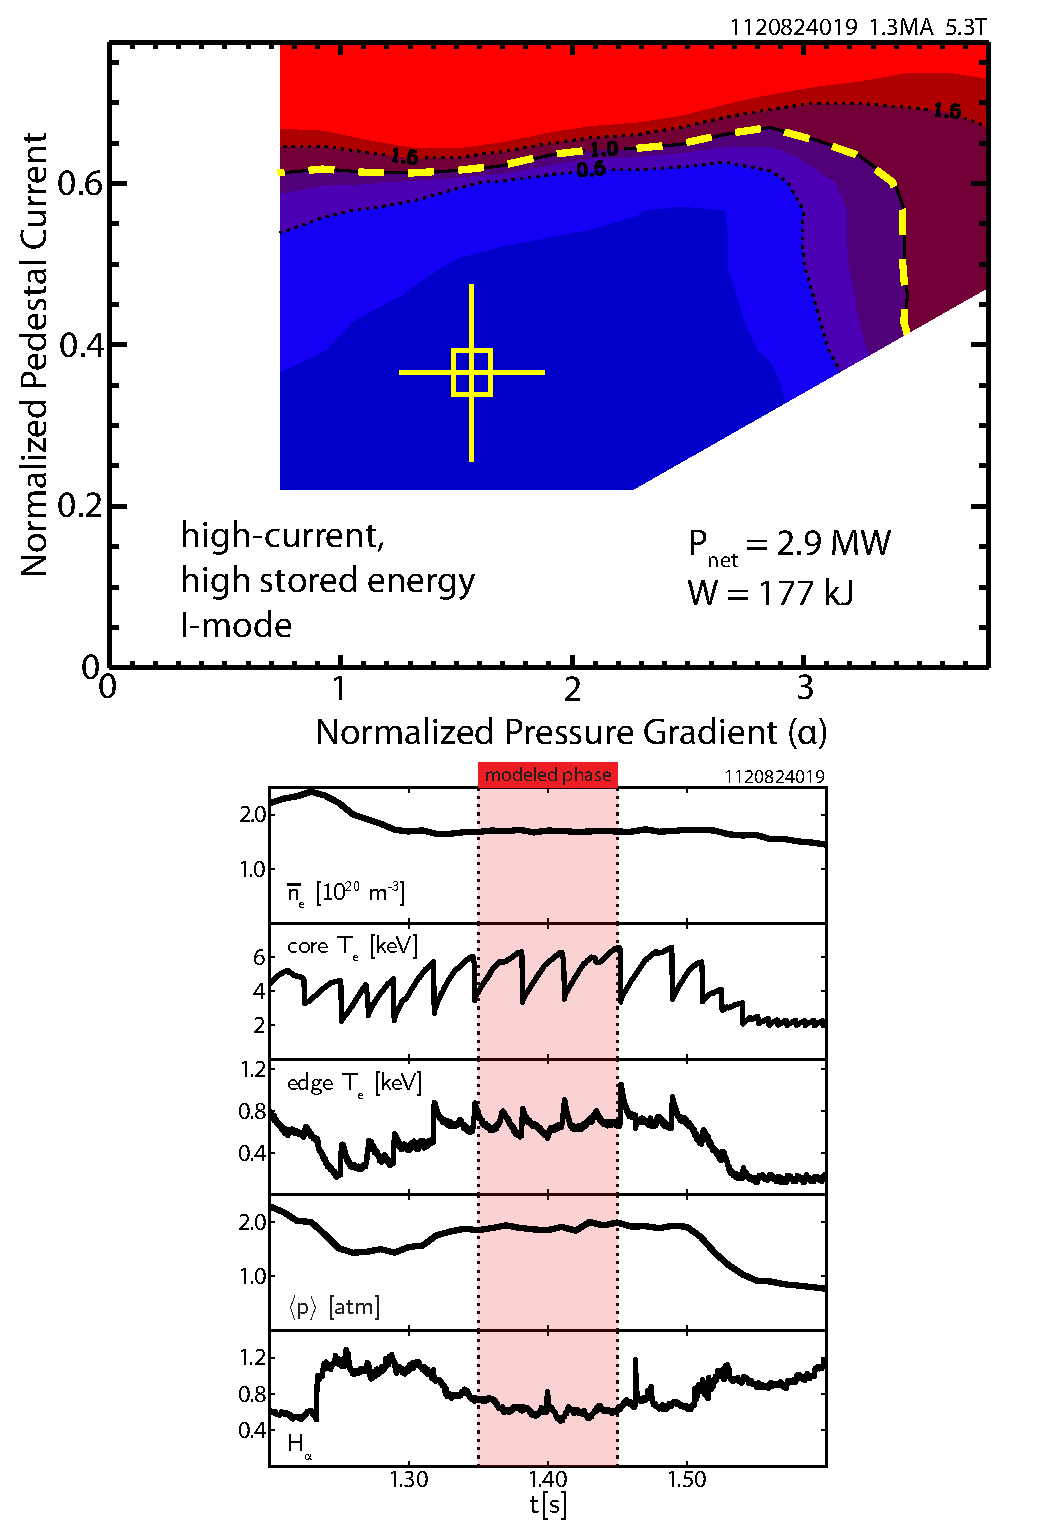
\includegraphics[width=150mm]{graphics/IModeModeling/1120824019_ELITE_stitch_vert.pdf}}{\caption[]{}\label{fig:imode_elite_noelm}}
\end{figure}

\begin{figure}[p]
 \pushtooutside
 \ffigbox[\FBwidth]{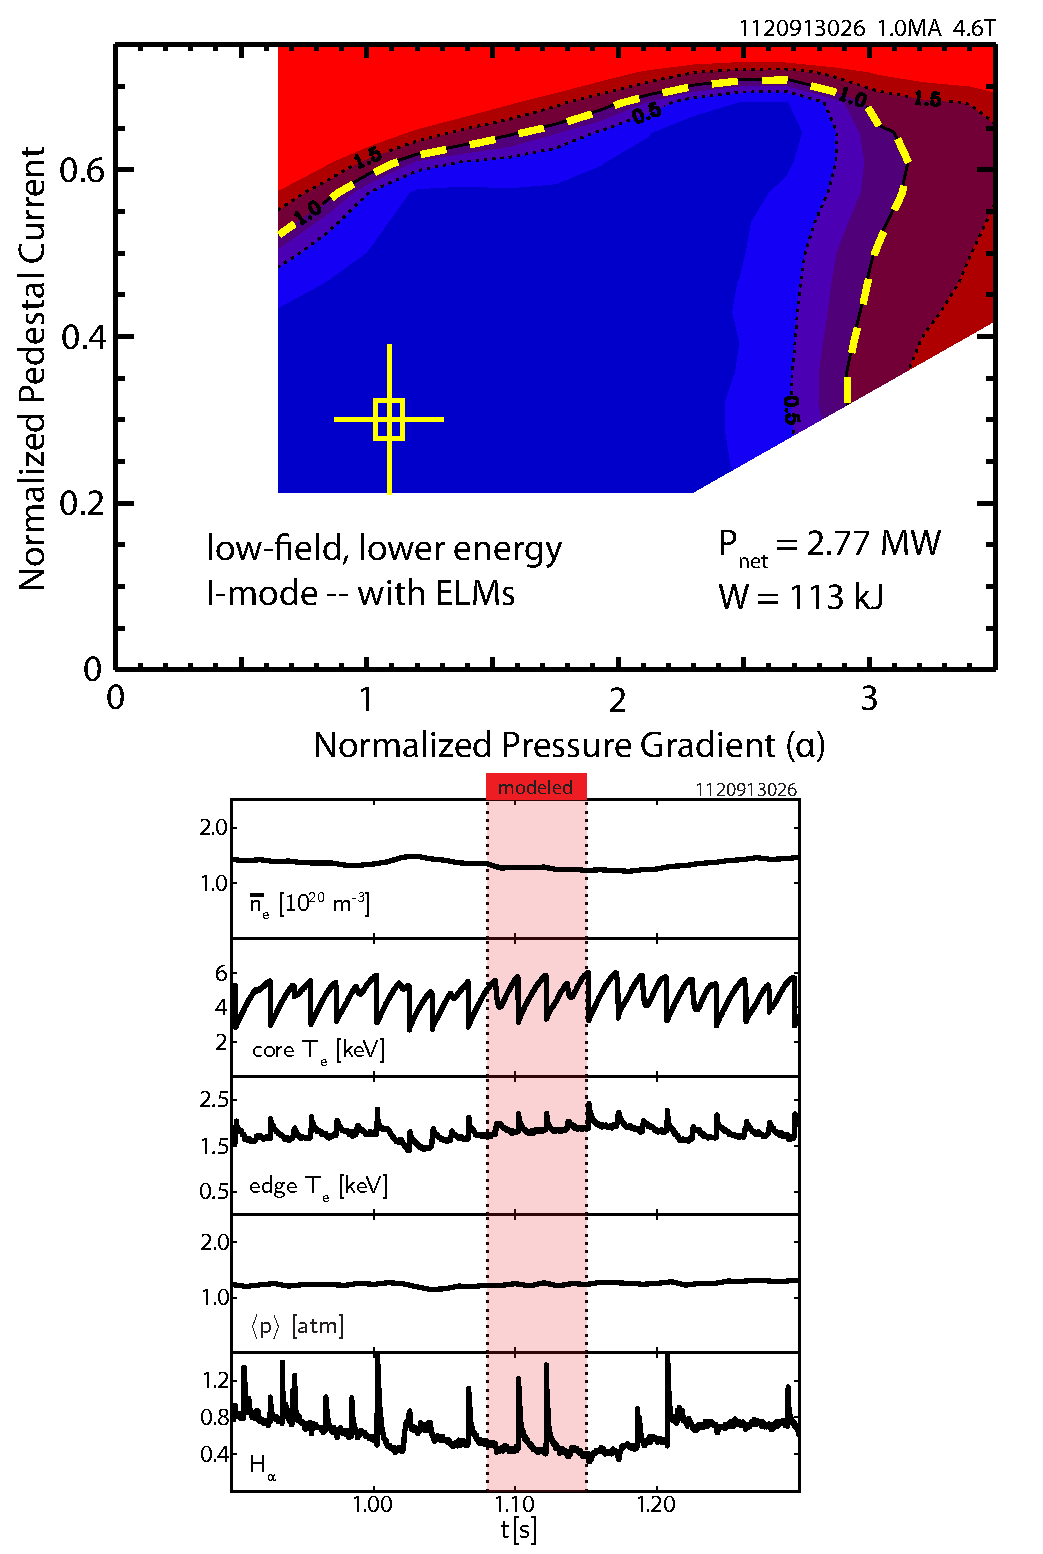
\includegraphics[width=150mm]{graphics/IModeModeling/1120913026_ELITE_stitch_vert.pdf}}{\caption[]{}\label{fig:imode_elite_stelm}}
\end{figure}

\begin{figure}
 \pushtooutside
 \ffigbox[\FBwidth]{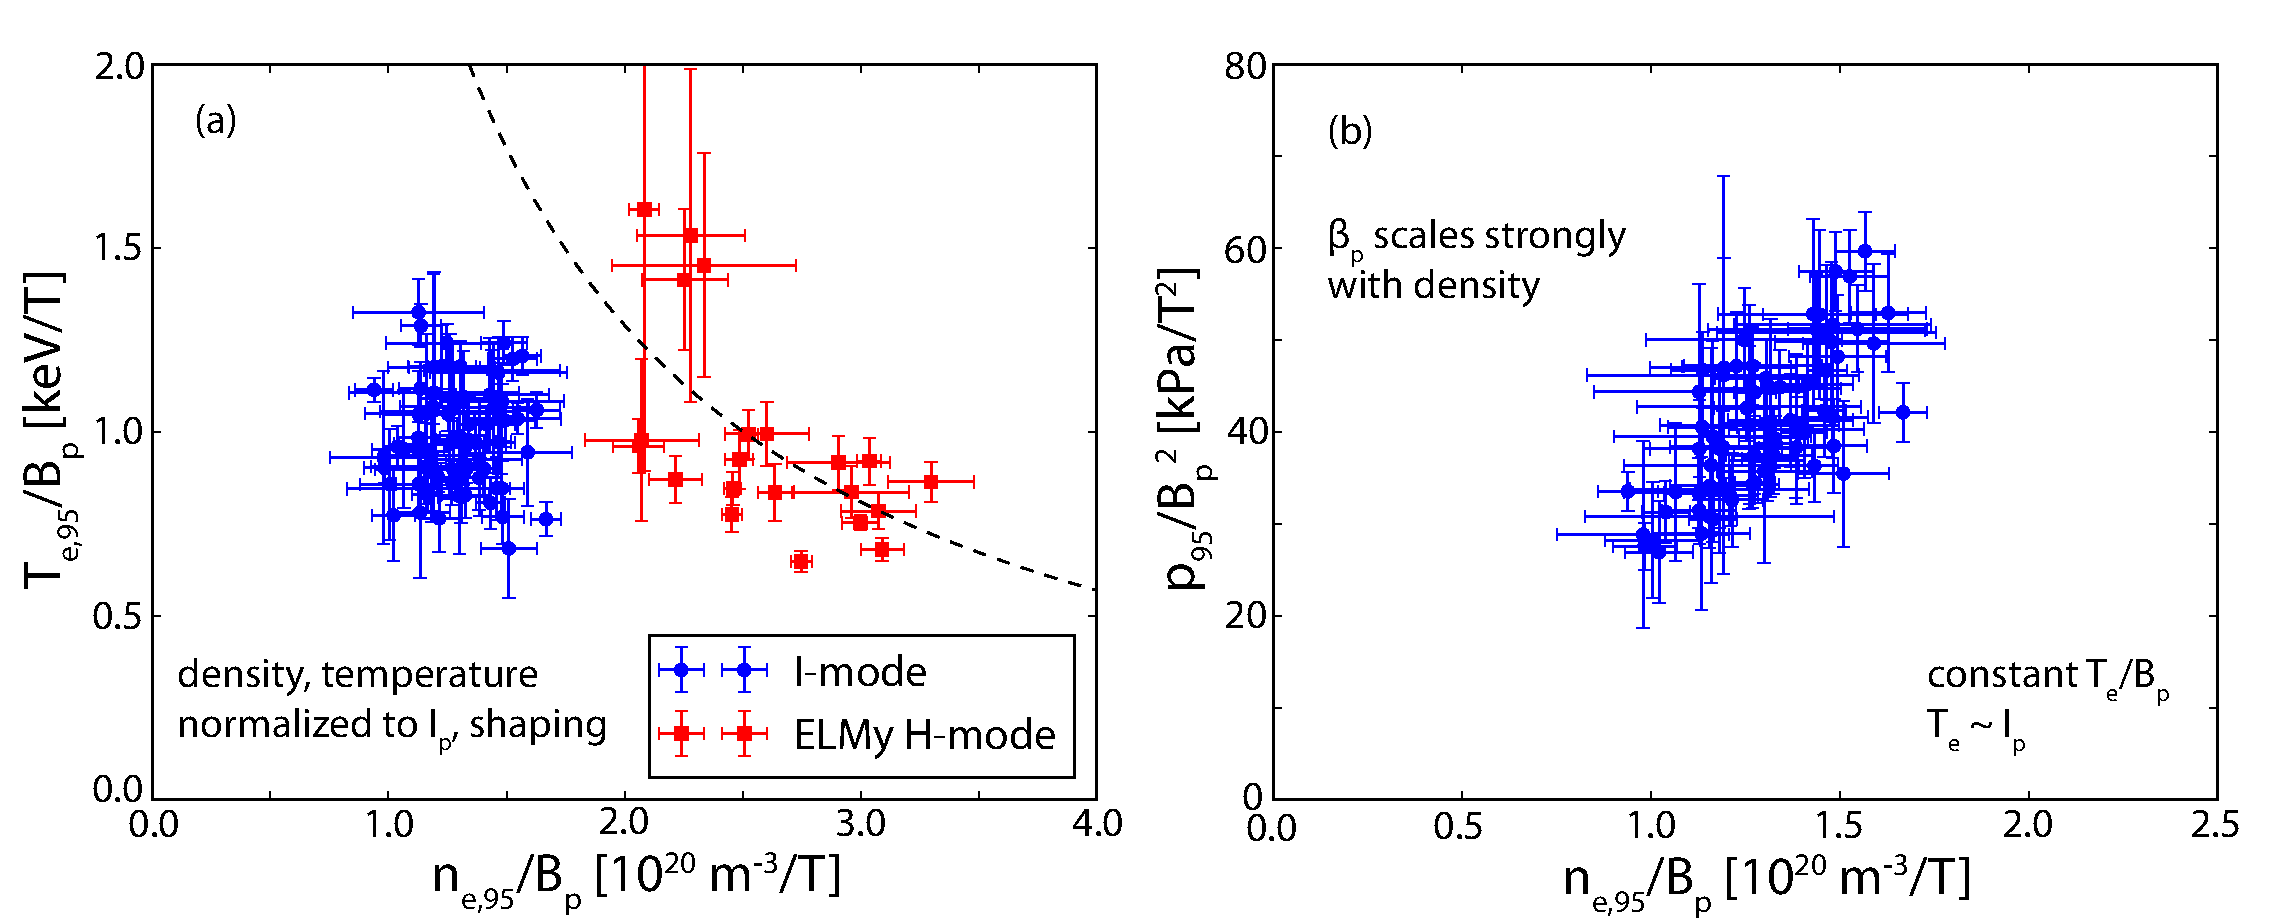
\includegraphics[width=150mm]{graphics/IModeModeling/neBp_stitch.pdf}}{\caption[]{}\label{fig:neBp_stitch}}
\end{figure}

\nicesectionending

\section{KBM and Infinite-$n$ MHD Stability}\label{sec:imode_baloo}

\begin{figure}
 \pushtooutside
 \ffigbox[\FBwidth]{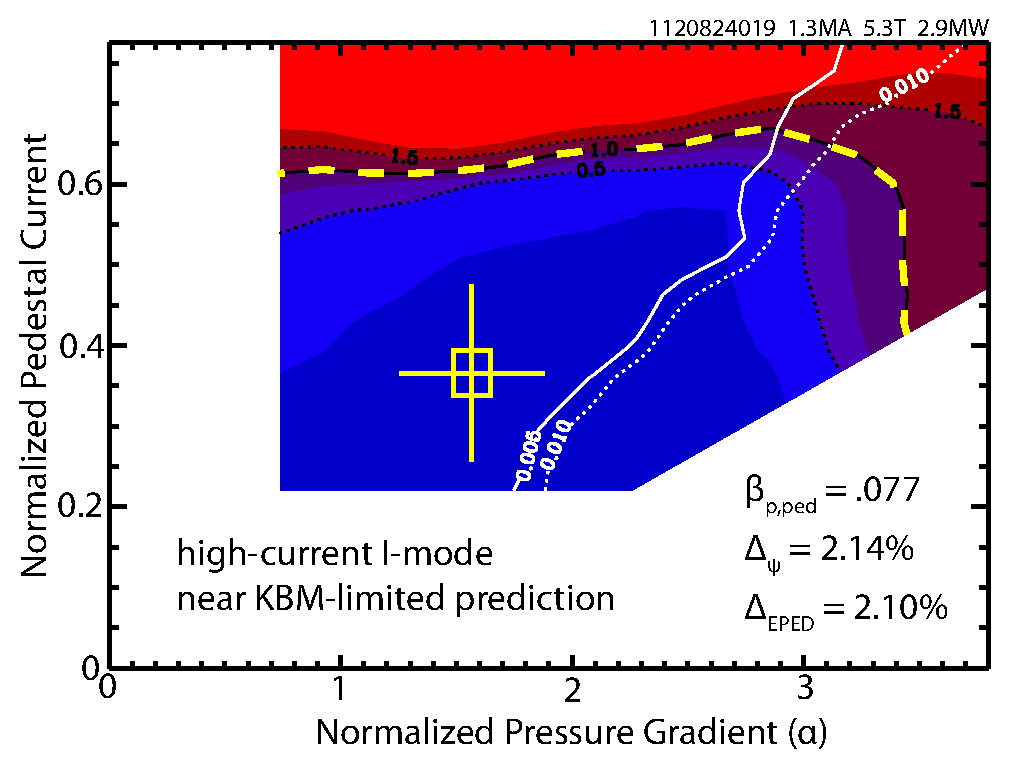
\includegraphics[width=150mm]{graphics/IModeModeling/1120824019_1400n5_35_gamws16_bal.pdf}}{\caption[]{}\label{fig:imode_baloo_noelm}}
\end{figure}

\begin{figure}
 \pushtooutside
 \ffigbox[\FBwidth]{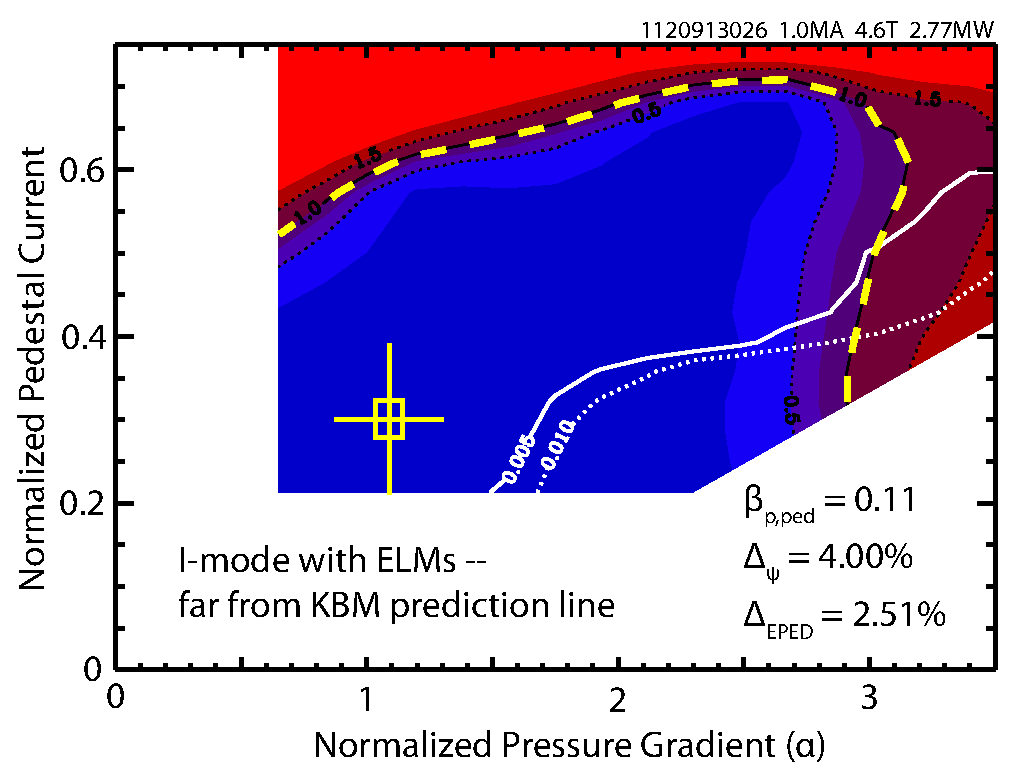
\includegraphics[width=150mm]{graphics/IModeModeling/1120913026_1186n5_35_bal_jalpha.pdf}}{\caption[]{}\label{fig:imode_baloo_stelm}}
\end{figure}

\nicesectionending

\section{Sawtooth Perturbations of Pedestal Stability}\label{sec:imode_sawtooth}

\begin{figure}
 \pushtooutside
 \ffigbox[\FBwidth]{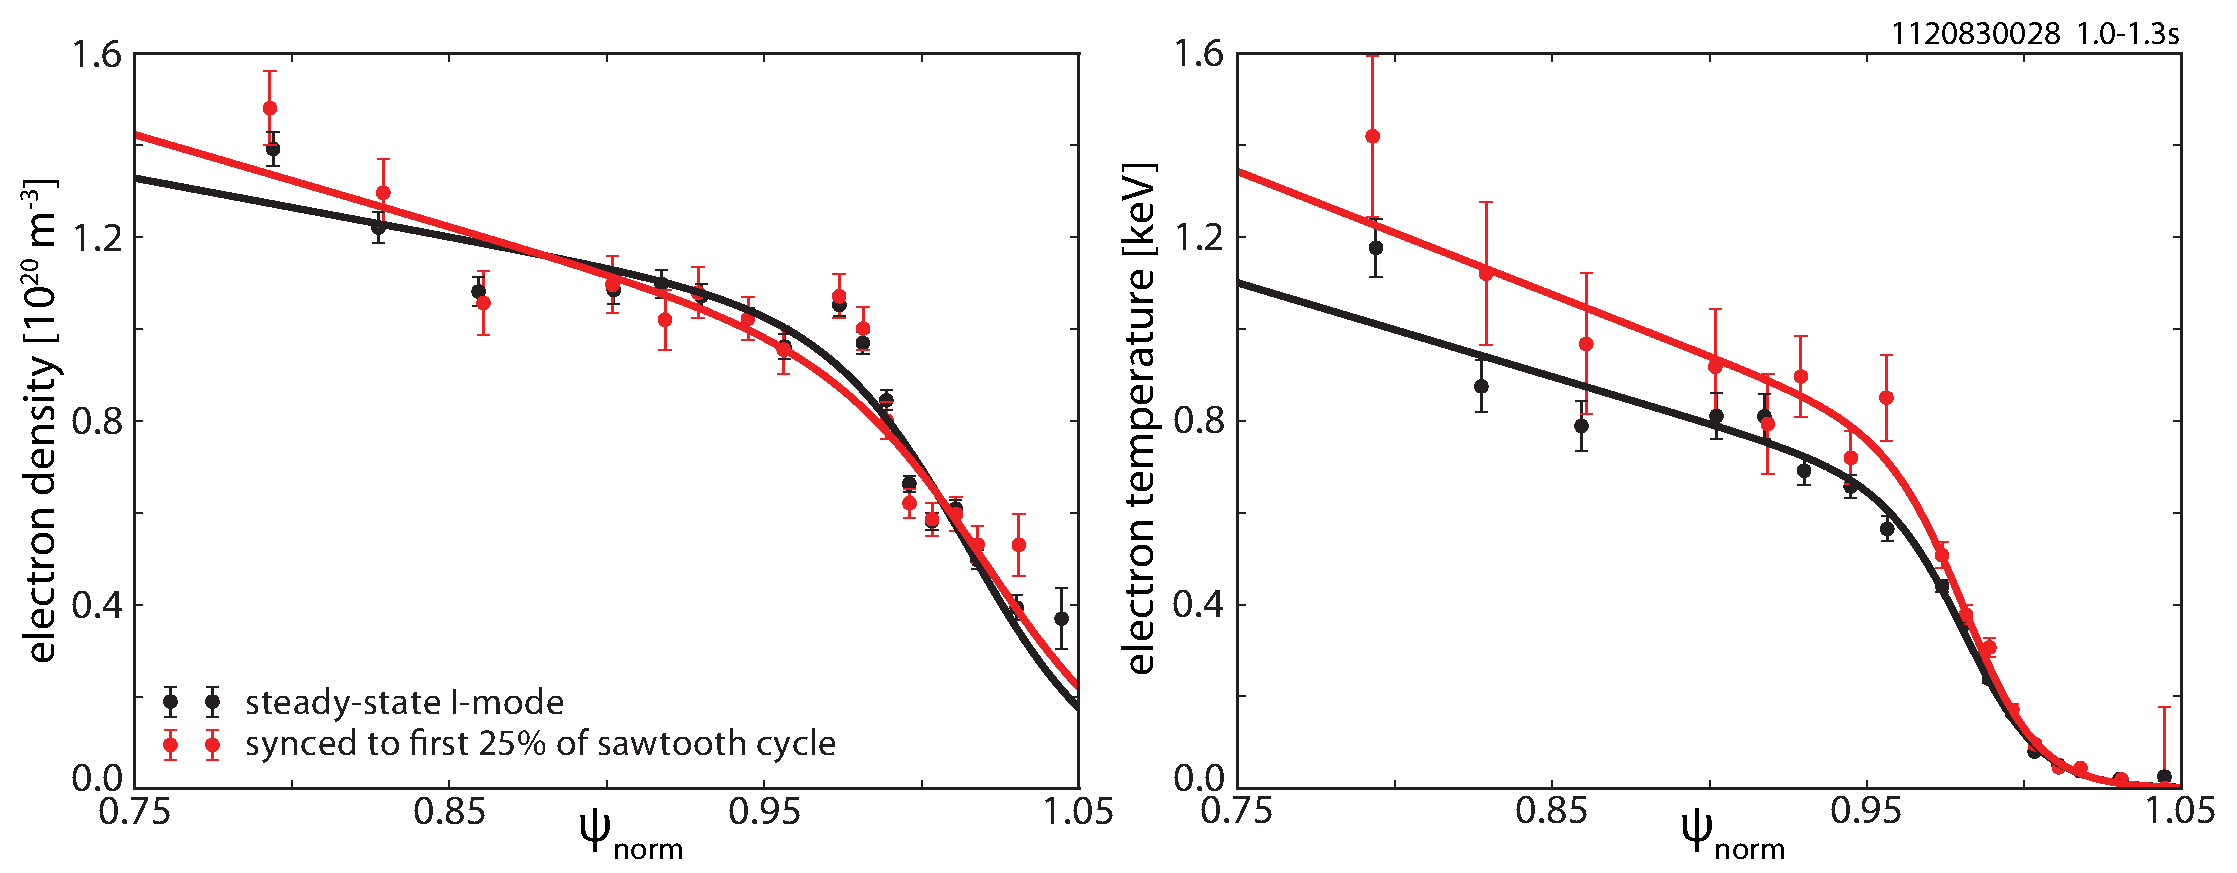
\includegraphics[width=150mm]{graphics/IModeModeling/1120830028_prof_stbin.pdf}}{\caption[]{}\label{fig:prof_stbin}}
\end{figure}

\begin{figure}
 \pushtooutside
 \ffigbox[\FBwidth]{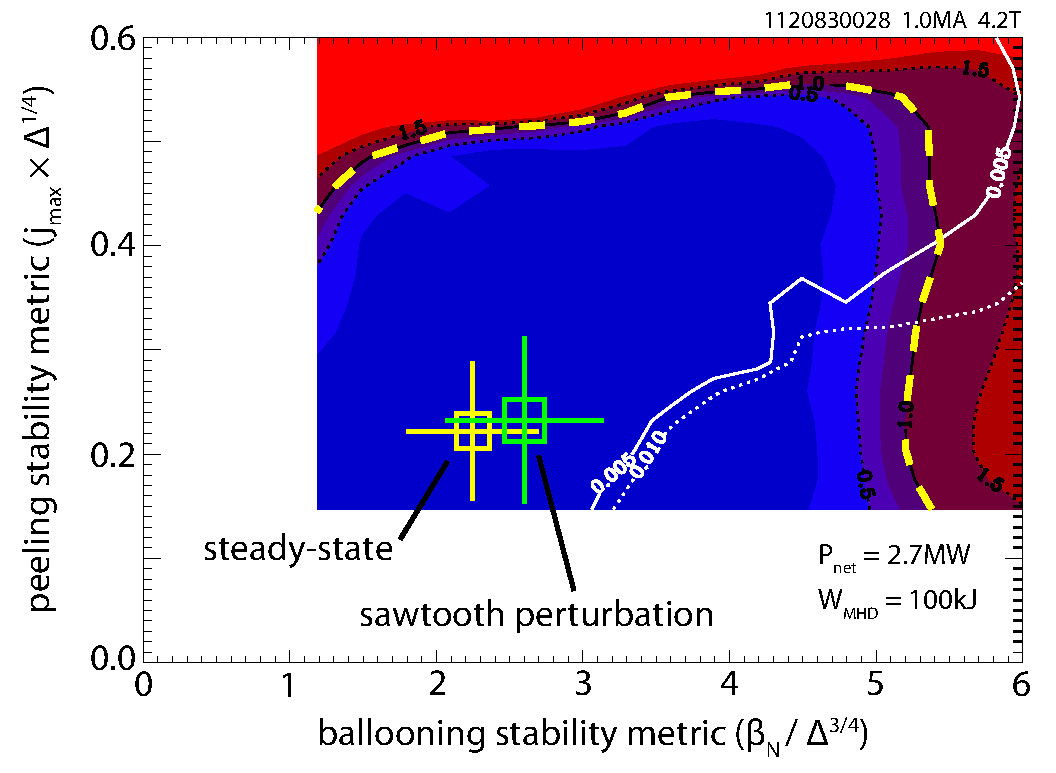
\includegraphics[width=150mm]{graphics/IModeModeling/1120830028_stbin_elite.pdf}}{\caption[]{}\label{fig:imode_stbin}}
\end{figure}

\nicesectionending

\section{ELM behavior}\label{sec:imode_elms}

\begin{figure}
 \pushtooutside
 \ffigbox[\FBwidth]{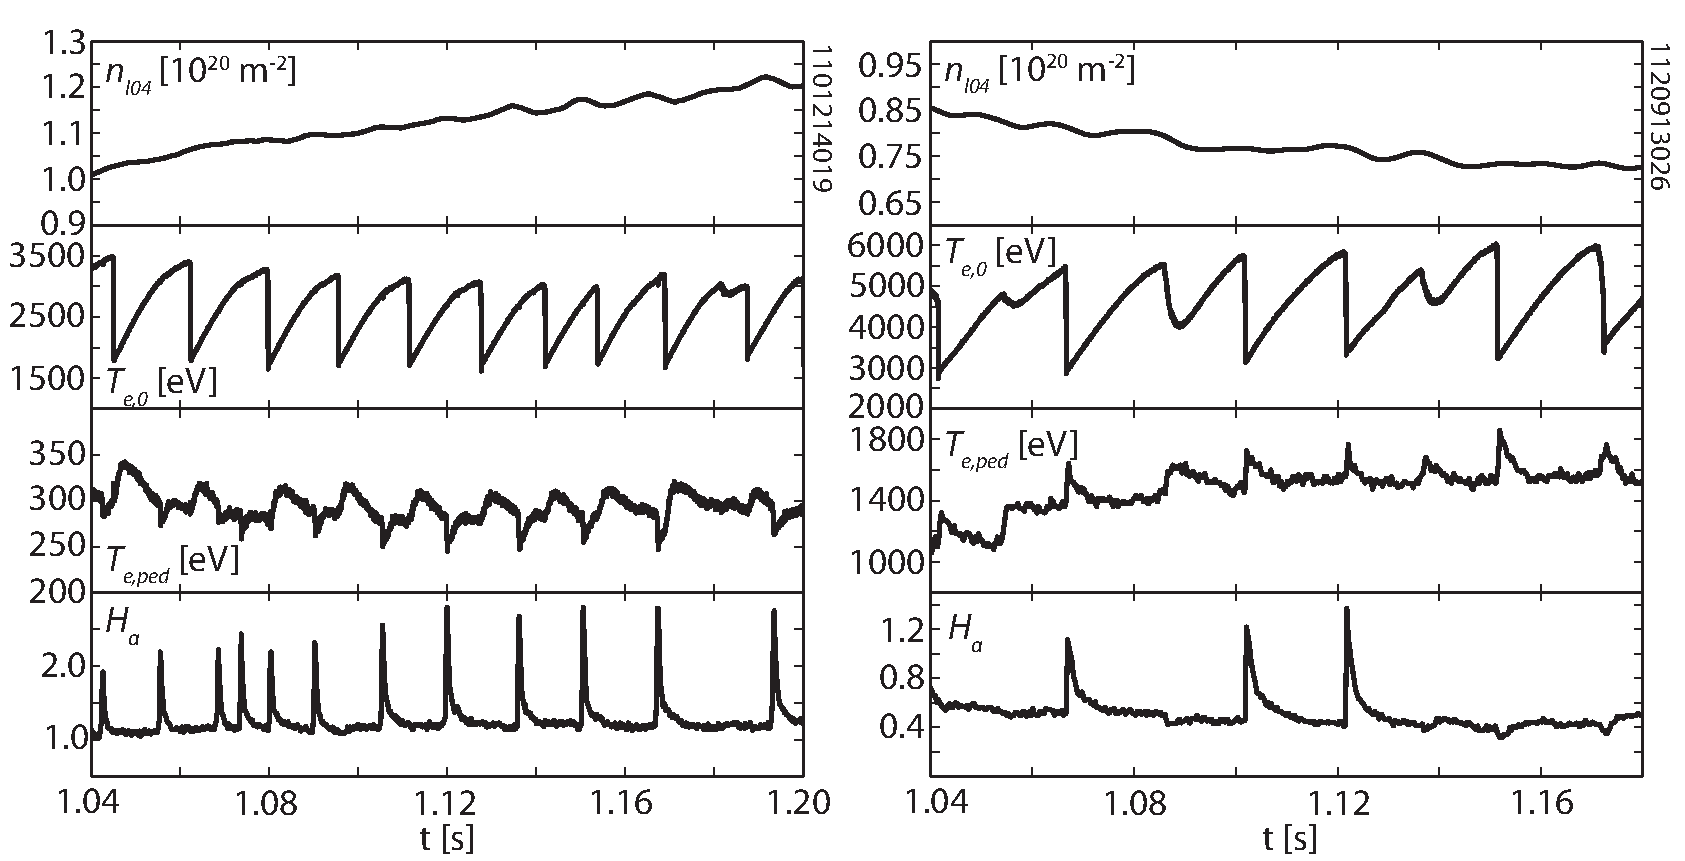
\includegraphics[width=150mm]{graphics/IModeModeling/trace_elmy_imode.pdf}}{\caption[]{}\label{fig:trace_elmy_imode}}
\end{figure}

\begin{figure}
 \pushtooutside
 \fcapside[60mm]{\caption[]{}\label{fig:trace_imode_welms}}{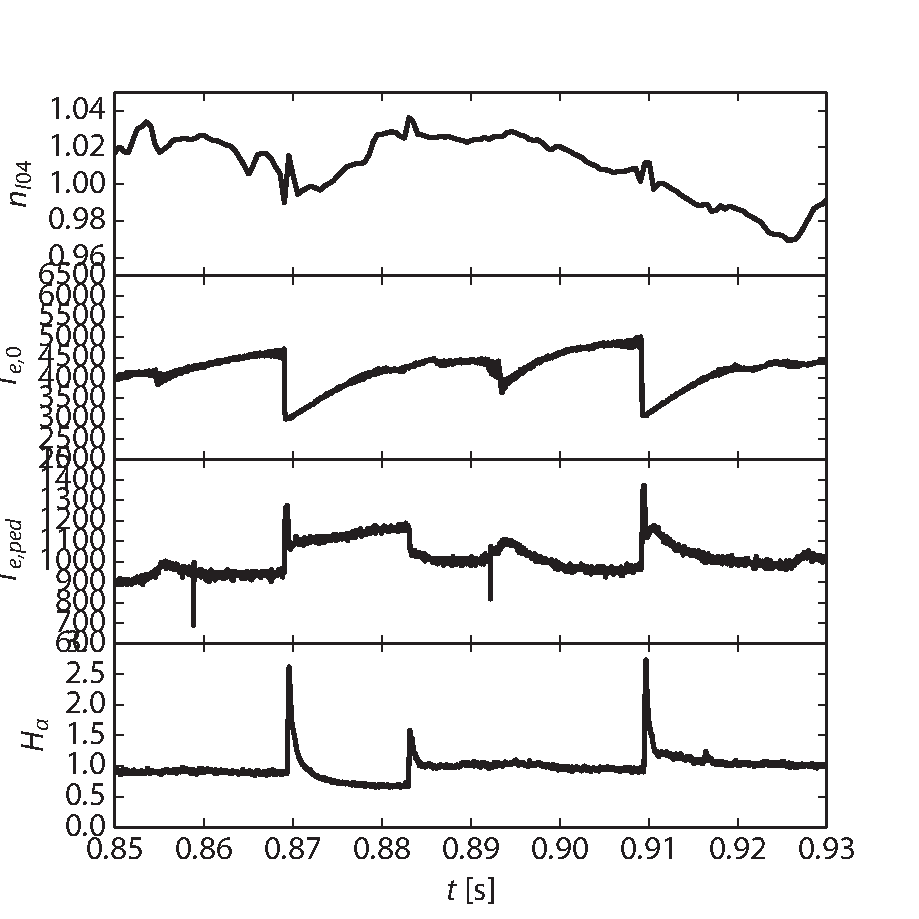
\includegraphics[width=100mm]{graphics/IModeModeling/trace_imode_welms_2.pdf}}
\end{figure}

\begin{figure}[p]
 \pushtooutside
 \ffigbox[\FBwidth]{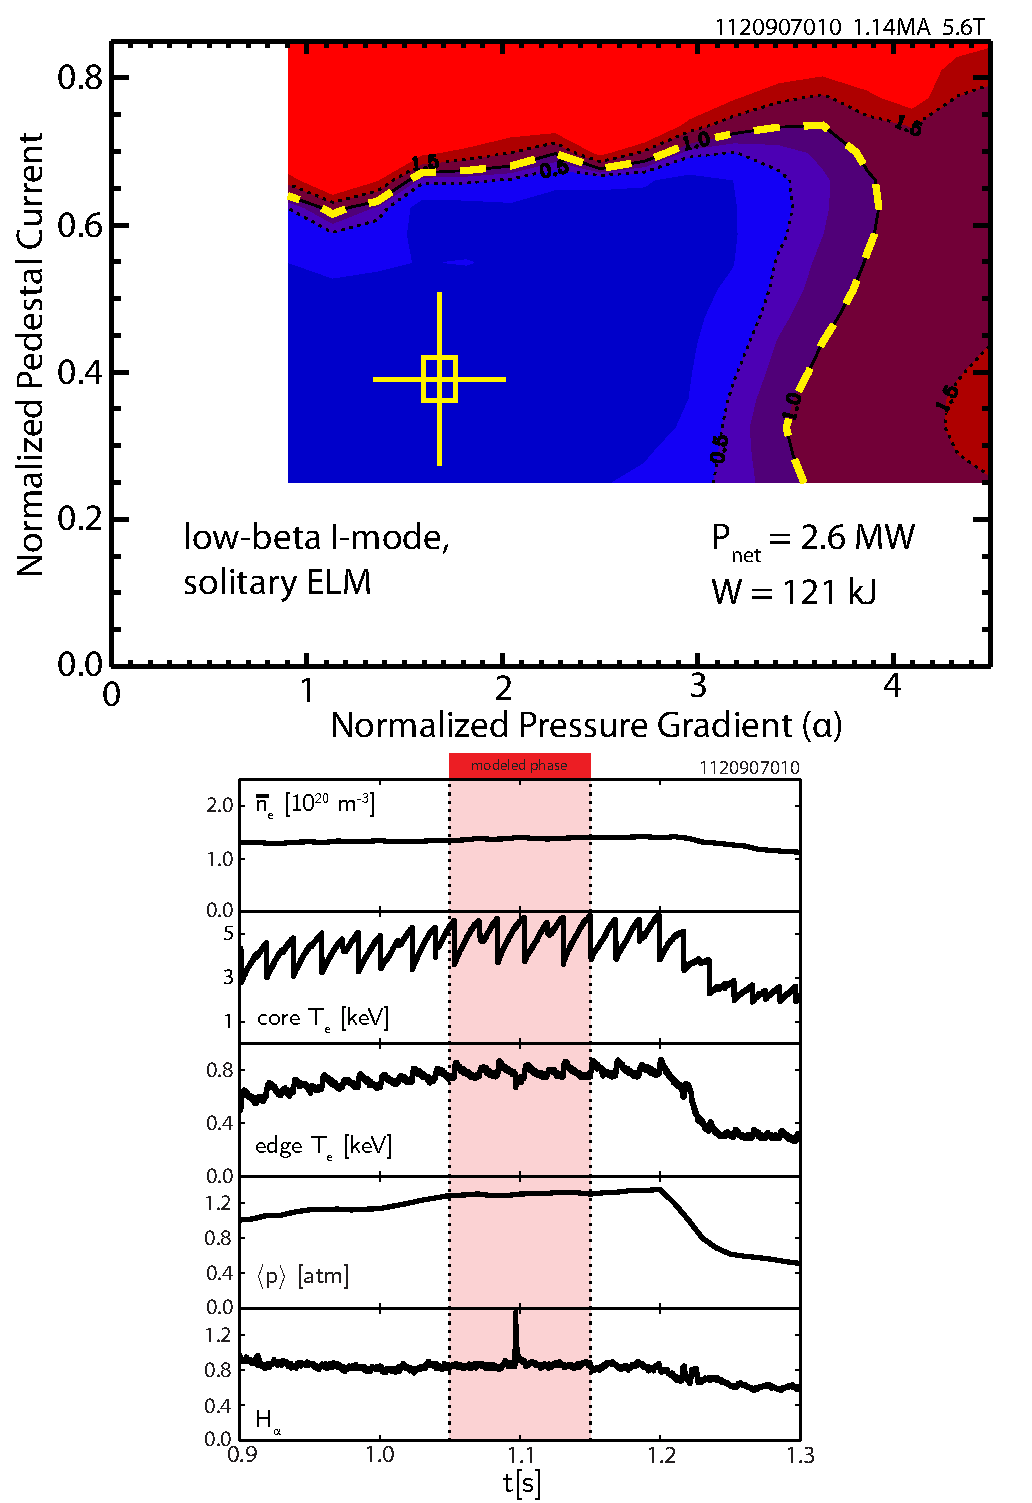
\includegraphics[width=150mm]{graphics/IModeModeling/1120907010_ELITE_stitch_vert.pdf}}{\caption[]{}\label{fig:imode_elite_nonstelms}}
\end{figure}

\begin{figure}
 \pushtooutside
 \ffigbox[\FBwidth]{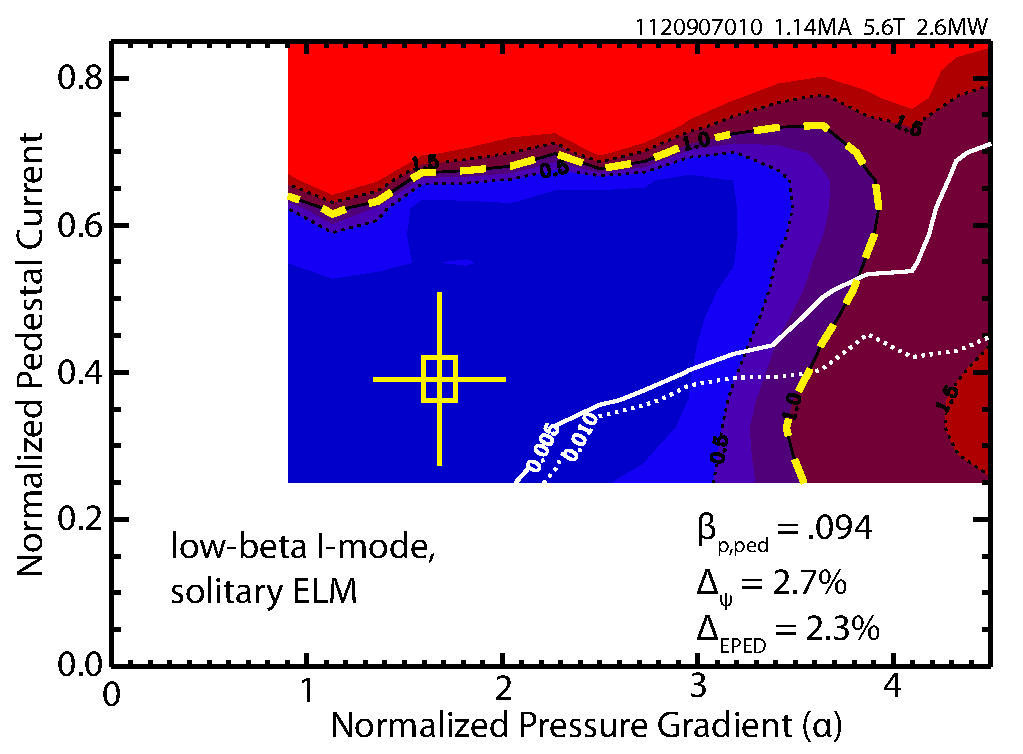
\includegraphics[width=150mm]{graphics/IModeModeling/1120907010_1100n5_35_gamws16_bal.pdf}}{\caption[]{}\label{fig:imode_baloo_nonstelms}}
\end{figure}

\nicechapterending

\bibliographystyle{../plainurl}
\bibliography{../references}